\frameT{Preferences Are Ubiquitous}{
	\begin{figure}[ht!]
	  \centering
	    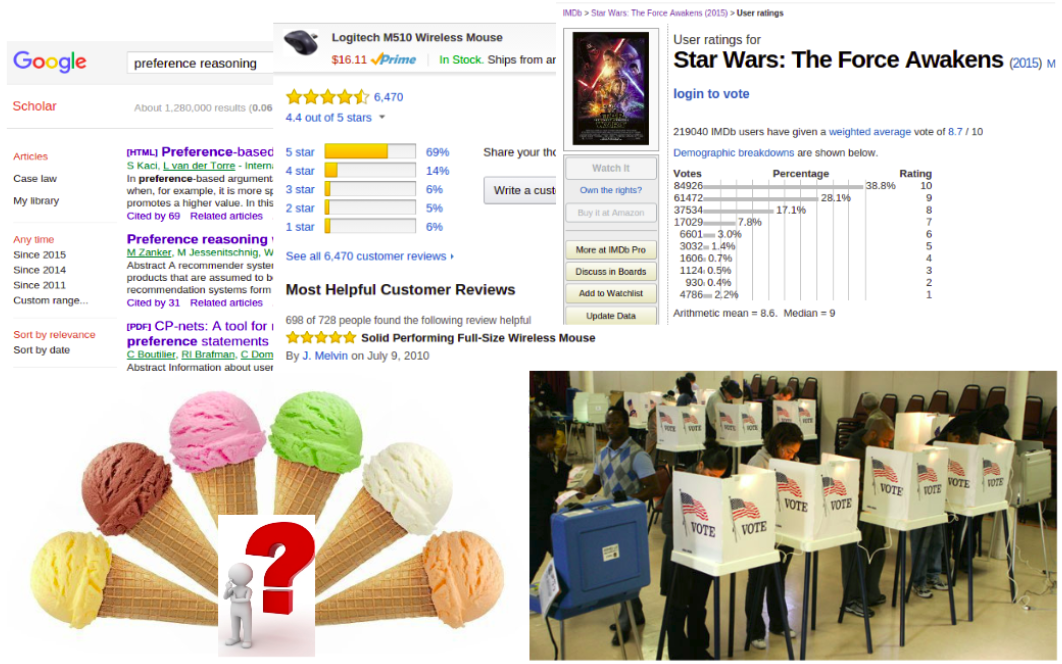
\includegraphics[width=0.8\textwidth]{figs/PrefApplications/pref_applications.png}
	  \caption{Preferences of different forms}
	\end{figure}
}

\frameT{Describing Preferences}{
	\begin{figure}[ht!]
	  \centering
	    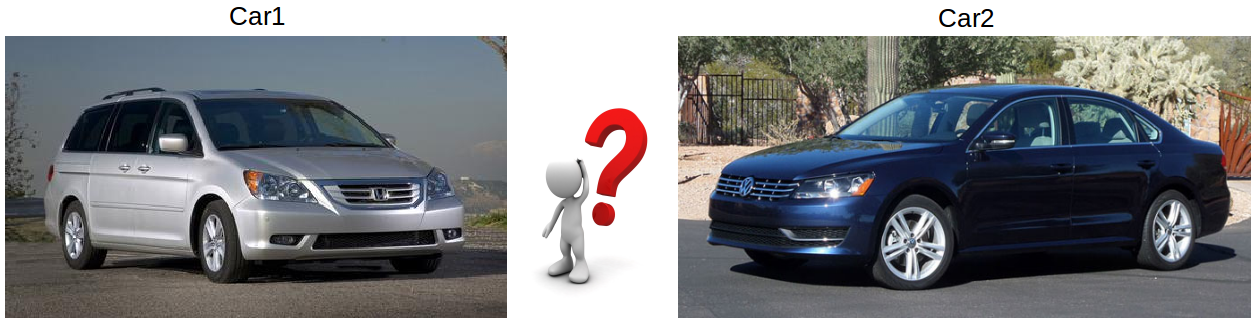
\includegraphics[width=0.95\textwidth]{figs/Cars/pref.png}
	  \caption{How to express preferences?}
	\end{figure}

	\vspace{-0.7cm}

	\begin{enumerate}
		\item On scale of 0 to 99, how will I rate these two cars?
		\begin{itemize}
			\item I give Car1 44 points and Car2 78 points; thus, I prefer Car2 to Car1.
		\end{itemize}
		\item Which one to me is better than the other?
		\begin{itemize}
			\item I prefer Car1 to Car2. (Strict preference)
			\item I like Car1 and Car2 equally. (Indifference/Equivalence)
			\item I cannot decide. (Incomparability)
		\end{itemize}
	\end{enumerate}
}

\frameT{Describing Preferences}{
	\begin{figure}[ht!]
	  \centering
	    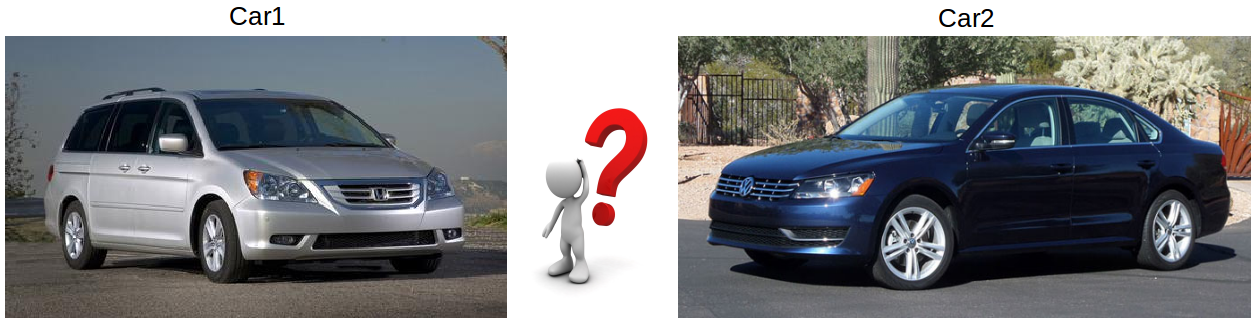
\includegraphics[width=0.95\textwidth]{figs/Cars/pref.png}
	  \caption{How to express preferences?}
	\end{figure}

	\vspace{-0.7cm}

	\begin{enumerate}
		\item On scale of 0 to 99, how will I rate these two cars? (\tbf{Quantitative})
		\begin{itemize}
			\item I give Car1 44 points and Car2 78 points; thus, I prefer Car2 to Car1.
		\end{itemize}
		\item Which one to me is better than the other? (\tbf{Qualitative})
		\begin{itemize}
			\item I prefer Car1 to Car2. (Strict preference)
			\item I like Car1 and Car2 equally. (Indifference/Equivalence)
			\item I cannot decide. (Incomparability)
		\end{itemize}
	\end{enumerate}
}
